\documentclass{report}
% Include all project wide packages here.
\usepackage{fullpage}
\usepackage[style=ieee]{biblatex}
\usepackage[dutch]{babel}

\renewcommand{\familydefault}{\sfdefault}

\setmainfont[Ligatures=TeX]{Myriad Pro}
\setmathfont{Asana Math}
\setmonofont{Lucida Console}

\usepackage{titlesec, blindtext, color}
\definecolor{gray75}{gray}{0.75}
\newcommand{\hsp}{\hspace{20pt}}
\titleformat{\chapter}[hang]{\Huge\bfseries}{\thechapter\hsp\textcolor{gray75}{|}\hsp}{0pt}{\Huge\bfseries}
\renewcommand{\familydefault}{\sfdefault}
\renewcommand{\arraystretch}{1.2}
\setlength\parindent{0pt}

%For code listings
\definecolor{black}{rgb}{0,0,0}
\definecolor{browntags}{rgb}{0.65,0.1,0.1}
\definecolor{bluestrings}{rgb}{0,0,1}
\definecolor{graycomments}{rgb}{0.4,0.4,0.4}
\definecolor{redkeywords}{rgb}{1,0,0}
\definecolor{bluekeywords}{rgb}{0.13,0.13,0.8}
\definecolor{greencomments}{rgb}{0,0.5,0}
\definecolor{redstrings}{rgb}{0.9,0,0}
\definecolor{purpleidentifiers}{rgb}{0.01,0,0.01}


\lstdefinestyle{csharp}{
language=[Sharp]C,
showspaces=false,
showtabs=false,
breaklines=true,
showstringspaces=false,
breakatwhitespace=true,
escapeinside={(*@}{@*)},
columns=fullflexible,
commentstyle=\color{greencomments},
keywordstyle=\color{bluekeywords}\bfseries,
stringstyle=\color{redstrings},
identifierstyle=\color{purpleidentifiers},
basicstyle=\ttfamily\small}

\lstdefinestyle{c}{
language=C,
showspaces=false,
showtabs=false,
breaklines=true,
showstringspaces=false,
breakatwhitespace=true,
escapeinside={(*@}{@*)},
columns=fullflexible,
commentstyle=\color{greencomments},
keywordstyle=\color{bluekeywords}\bfseries,
stringstyle=\color{bluestrings},
identifierstyle=\color{purpleidentifiers}
}

\lstdefinestyle{vhdl}{
language=VHDL,
showspaces=false,
showtabs=false,
breaklines=true,
showstringspaces=false,
breakatwhitespace=true,
escapeinside={(*@}{@*)},
columns=fullflexible,
commentstyle=\color{greencomments},
keywordstyle=\color{bluekeywords}\bfseries,
stringstyle=\color{redstrings},
identifierstyle=\color{purpleidentifiers}
}

\lstdefinestyle{xaml}{
language=XML,
showspaces=false,
showtabs=false,
breaklines=true,
showstringspaces=false,
breakatwhitespace=true,
escapeinside={(*@}{@*)},
columns=fullflexible,
commentstyle=\color{greencomments},
keywordstyle=\color{redkeywords},
stringstyle=\color{bluestrings},
tagstyle=\color{browntags},
morestring=[b]",
  morecomment=[s]{<?}{?>},
  morekeywords={xmlns,version,typex:AsyncRecords,x:Arguments,x:Boolean,x:Byte,x:Char,x:Class,x:ClassAttributes,x:ClassModifier,x:Code,x:ConnectionId,x:Decimal,x:Double,x:FactoryMethod,x:FieldModifier,x:Int16,x:Int32,x:Int64,x:Key,x:Members,x:Name,x:Object,x:Property,x:Shared,x:Single,x:String,x:Subclass,x:SynchronousMode,x:TimeSpan,x:TypeArguments,x:Uid,x:Uri,x:XData,Grid.Column,Grid.ColumnSpan,Click,ClipToBounds,Content,DropDownOpened,FontSize,Foreground,Header,Height,HorizontalAlignment,HorizontalContentAlignment,IsCancel,IsDefault,IsEnabled,IsSelected,Margin,MinHeight,MinWidth,Padding,SnapsToDevicePixels,Target,TextWrapping,Title,VerticalAlignment,VerticalContentAlignment,Width,WindowStartupLocation,Binding,Mode,OneWay,xmlns:x}
}

%defaults
\lstset{
basicstyle=\ttfamily\small,
extendedchars=false,
numbers=left,
numberstyle=\ttfamily\tiny,
stepnumber=1,
tabsize=4,
numbersep=5pt
}
\addbibresource{../../library/bibliography.bib}

\title{EPO-2: Mid-term Design Report - Mijndetector}
\author{Chy Lau}

\begin{document}

\chapter{Mijndetector}
\label{ch:mijn}
Om een mijndetector op te bouwen, moet er eerst een keuze worden gemaakt tussen de verschillende soorten sensoren. Maken we gebruik van een inductieve sensor, capacitieve sensor of een combinatie van beiden?

Wij hebben uiteindelijk voor de inductieve sensor gekozen. De inductieve sensor gebruikt minder componenten dan de capacitieve sensor. Dus de inductieve sensor heeft qua opbouw het meest eenvoudige circuit. De werking van deze sensor is dan ook makkelijker te verklaren. 

\section{Eisen}
\label{sec:eisen}
De mijn-detecterende sensor moet aan de volgende eisen voldoen: 
\begin{itemize}
\item De mijndetector moet een metalen ring detecteren op het wedstrijdveld;
\item De sensor mag geen contact maken met de metalen ring;
\item De sensor moet compatibel met de batterij op de robot zijn; 
\item Het uitgangssignaal van de sensor is een blokgolf;
\end{itemize}

\section{Ontwerp}
\label{sec:ontwerp}
De schakeling van de inductieve sensor is zoals die van de JIT: Inductieve sensoren. Het is overbodig om de schakeling te veranderen, want de originele schakeling levert geen problemen op. In figuur \ref{fig:schakeling_sensor} staat de oscillator op basis van de inductieve sensor.

\subsection{Werkingsprincipe}
\label{ssec:werking}
Over het algmeen zijn er twee mogelijke werkingsprincipes voor de inductieve sensor. De eerste werkt op basis van de verandering van permeabiliteit. De tweede werkt op basis van een pulserend veld. 

Voor de sensor geldt de eerste werkingsprincipe. Er zal een verschil van permeabiliteit gedetecteerd worden, omdat lucht een andere permeabiliteit heeft dan metaal. De magnetische veldlijnen uit de spoel zullen veranderd worden wanneer ze door het metaal heen gaan. Dit leidt ertoe dat de inductiviteit van de spoel verandert. Deze verandering kan worden weergegeven in een periodiek signaal.

\newpage
\subsection{Werking}

Het circuit dat gebruikt wordt voor de inductieve sensor is een LC-circuit. Hiermee kan de resonantiefrequentie veranderd worden, zodat het uitgangssignaal van de schakeling ook verandert.

\begin{figure}[H]
\centering
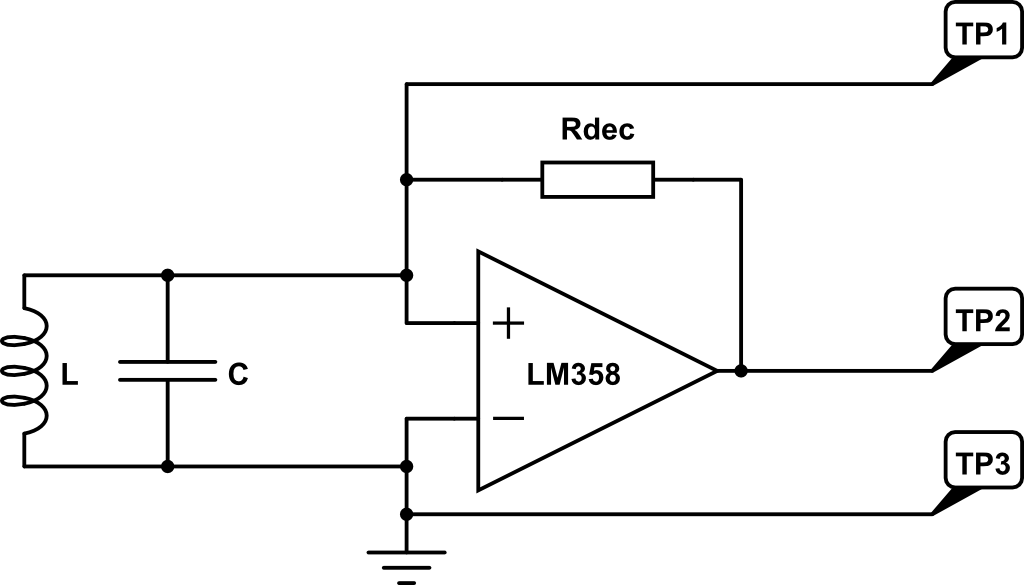
\includegraphics[scale=0.45]{inductieve_sensor.png}
\caption{Schakeling van de inductieve sensor.}
\label{fig:schakeling_sensor}
\end{figure}

\subsubsection{LC-circuit}
Een belangrijke eigenschap van het circuit is de resonantiefrequentie. Om de $f_res$ te begrijpen is het van belang om naar het gedrag van de elektronen te kijken. De elektronen schommelen steeds heen en weer, van de ene kant van de condensator-plaat naar de andere kant van de condensator-plaat. Hoe snel zo een schommeling gaat, wordt uitgedrukt als de resonantiefrequentie. Deze frequentie hangt af van de spoel en condensator die wordt gebruikt in het circuit. Met de volgende formule kan de $f_{res}$ worden berekend:

\begin{equation}
f_{res}=\frac{1}{2\pi\sqrt{LC}}
\end{equation}

\subsubsection{Comparator}
De comparator is een essentieel onderdeel van de schakeling. Het zorgt ervoor dat er op een uitgang een blokgolf komt te staan. Zo een blokgolf kan dan getransformeerd worden in een logisch signaal van '0' en '1'. De comparator werkt als volgt:

\begin{equation}
Als \;V_+>V_- \Rightarrow V_{out}\approx V_{CC}
\end{equation}
\begin{equation}
Als \; V_+<V_- \Rightarrow V_{out}\approx V_{EE}
\end{equation}

Dit leidt ertoe dat de uitgangsspanning een zeer positieve- en negatieve waarde kan hebben. Deze schommeling van positief en negatief geeft uiteindelijk een blokgolf.\\

Dus doordat de resonantiefrequentie verandert wanneer de magnetische veldlijnen door het metaal heen gaan (L krijgt dan een andere waarde), zal ook de frequentie van het bloksignaal veranderen. 

\section{Implementatie}

\section{Test}

\section{Discussie}


\end{document}